%% --------------------------------------------------------------------------
% LaTeX template for the XLI CILAMCE.
%
% This latex document tries to copy the Microsoft Word template.
% --------------------------------------------------------------------------
\documentclass[a4paper,10pt]{book}

% PACKAGES USED - packages that need to be previously installed on your computer
\usepackage[lmargin=2.5cm, rmargin=2.5cm, tmargin=2.5cm, bmargin=2.5cm ]{geometry}
\usepackage{graphicx}
\usepackage{times}
\usepackage{indentfirst}
\usepackage{fancyhdr}
\usepackage{titlesec}
\usepackage[english]{babel}
\usepackage{parskip} 
\usepackage{setspace}



%%%%%%%%%%%%%%%%%%%%%%%%%%%%%%%%%%%%%%%%%%%%%%%%%%%%%%%%%%%%%%%%%
%%%%%%%%%%%%%%%%%%%%%%%%%%%%%%%%%%%%%%%%%%%%%%%%%%%%%%%%%%%%%%%%%
%%% My Additional Packages
%%%%%%%%%%%%%%%%%%%%%%%%%%%%%%%%%%%%%%%%%%%%%%%%%%%%%%%%%%%%%%%%%
\usepackage[utf8]{inputenc}
%\usepackage{amssymb} %Mathematics
%\usepackage{amsfonts}%Mathematics
%\usepackage{amsmath,amscd}%Mathematics
%\usepackage{amsthm}%Mathematics
%\usepackage{mathrsfs}%Mathematics font
%\usepackage{xspace}
%\usepackage{booktabs}
%\usepackage{stmaryrd}%Particular Brackets
%\usepackage{graphicx} %Tables and Figures
%\usepackage{subfigure}
%\usepackage{url}
\usepackage{hyperref}
\usepackage{cleveref}
\usepackage{./pkg-crefNames}
\usepackage[labelsep=period]{caption}

%BibTeX compatible with the CILAMCE format
\usepackage[numbers,sort&compress]{natbib}

\setlength{\bibsep}{0pt plus 0.3ex}

\renewcommand*{\bibfont}{\small}

\makeatletter
\renewcommand\bibsection
{
  \section*{References}
}



\renewenvironment{thebibliography}[1]
      {\section*{\refname}%
       \@mkboth{\MakeUppercase\refname}{\MakeUppercase\refname}%
       \list{\@biblabel{\@arabic\c@enumiv}}%
            {\settowidth\labelwidth{\@biblabel{#1}}%
             \leftmargin\labelwidth
             \advance\leftmargin-10pt% change 20 pt according to your needs
             \advance\leftmargin\labelsep
             \setlength\itemindent{10pt}% change using the inverse of the length used before
             \@openbib@code
             \usecounter{enumiv}%
             \let\p@enumiv\@empty
             \renewcommand\theenumiv{\@arabic\c@enumiv}}%
       \sloppy
       \clubpenalty4000
       \@clubpenalty \clubpenalty
       \widowpenalty4000%
       \sfcode`\.\@m}
      {\def\@noitemerr
        {\@latex@warning{Empty `thebibliography' environment}}%
       \endlist}
\renewcommand\newblock{\hskip .11em\@plus.33em\@minus.07em}
\makeatother




\makeatother
\bibliographystyle{./bib-cilamce}
%\bibliographystyle{plain}


%%%%%%%%%%%%%%%%%%%%%%%%%%%%%%%%%%%%%%%%%%%%%%%%%%%%%%%%%%%%%%%%%
%%%%%%%%%%%%%%%%%%%%%%%%%%%%%%%%%%%%%%%%%%%%%%%%%%%%%%%%%%%%%%%%%

% CONFIGURATION
\renewcommand*\arraystretch{1.5}
\renewcommand*\thesection{\arabic{section}}
%\hyphenpenalty=10000 % You can uncomment this to avoid hyphenization
\titleformat*{\section}{\large\bfseries}
\titleformat*{\subsection}{\bfseries}
\titlespacing\section{0pt}{20pt plus 2pt minus 2pt}{12pt plus 2pt minus 2pt}
\titlespacing\subsection{0pt}{20pt plus 0pt minus 0pt}{12pt plus 0pt minus 0pt}
\setlength{\parskip}{0pt} % Spacing between paragraphs
\setlength{\parindent}{0.75cm} % Paragraph identation
\setlength\abovecaptionskip{6pt}

% --------------------------------------------------------------------------
% DO NOT EDIT - SPECIAL HEADINGS OF XLI CILAMCE
% --------------------------------------------------------------------------
\fancypagestyle{first}
{
\fancyhf{}
\fancyfoot[RO]{\footnotesize \textit{CILAMCE 2020 \\
Proceedings of the XLI Ibero-Latin-American Congress on Computational Methods in Engineering, ABMEC.\\
Foz do Iguaçu/PR, Brazil, November 16-19, 2020}}
\renewcommand{\headrulewidth}{.0pt}
\renewcommand{\footrulewidth}{.5pt}
}

\pagestyle{fancy}
\fancyhf{}
\fancyhead[RO,LE]{}

\fancyfoot[RO]{\footnotesize \textit{CILAMCE 2020 \\
Proceedings of the XLI Ibero-Latin-American Congress on Computational Methods in Engineering, ABMEC.\\
Foz do Iguaçu/PR, Brazil, November 16-19, 2020}}

\fancyfoot[LE]{\footnotesize \textit{CILAMCE 2020 \\
Proceedings of the XLI Ibero-Latin-American Congress on Computational Methods in Engineering, ABMEC.\\
Foz do Iguaçu/PR, Brazil, November 16-19, 2020}}

\renewcommand{\headrulewidth}{.5pt}
\renewcommand{\footrulewidth}{.5pt}

% --------------------------------------------------------------------------
% PLEASE, EDIT THIS!
\fancyhead[LE]{\footnotesize \textit{Template for CILAMCE 2020 Concrete compressive strength prediction with machine learning}}
\fancyhead[RO]{\footnotesize \textit{P. Moreira, V. Silva}}
% --------------------------------------------------------------------------

\begin{document}\thispagestyle{first}

% --------------------------------------------------------------------------
% DO NOT EDIT - LOGO OF XLI CILAMCE
% --------------------------------------------------------------------------

\begin{figure}[ht!]
\vspace{-30pt}
\flushright
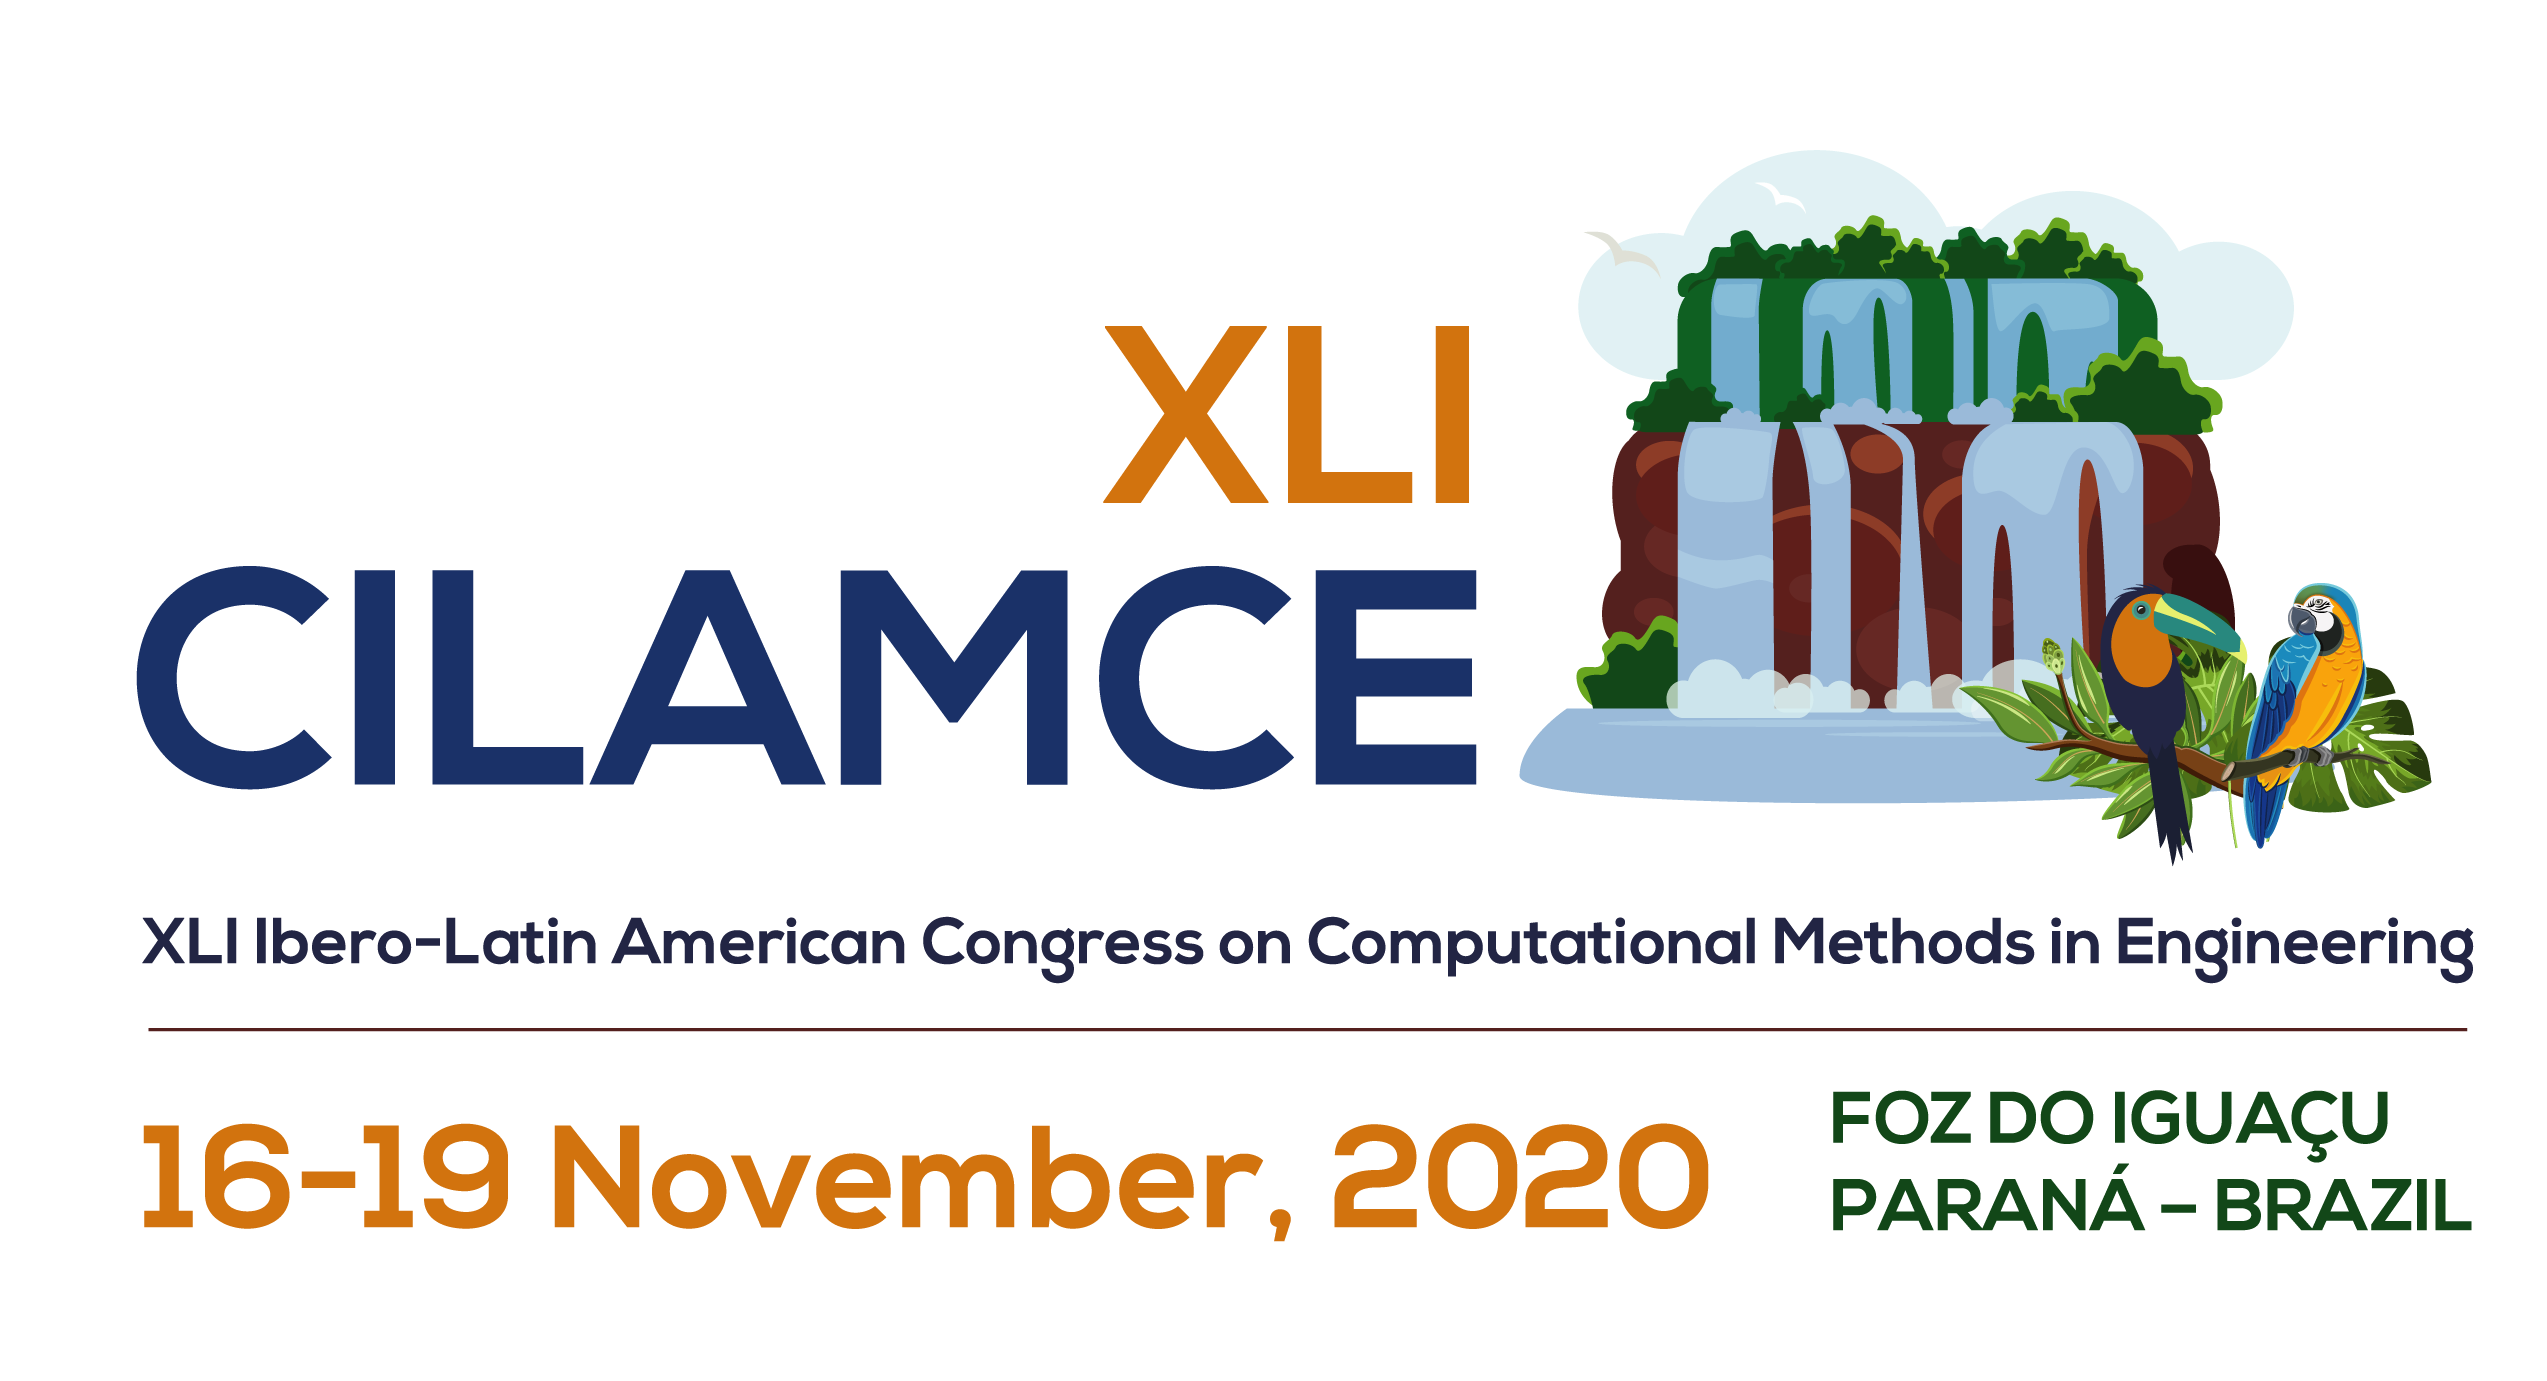
\includegraphics[width=5.5cm]{Figures/logoCILAMCE2020.png}
%scale=0.25
\end{figure}

% --------------------------------------------------------------------------
% TITLE OF PAPER
% --------------------------------------------------------------------------

\noindent
\textbf{\Large
Concrete compressive strength prediction with machine learning} 
\vspace{18pt} % <- keep this vertical space!

% --------------------------------------------------------------------------
% AUTHORS
% --------------------------------------------------------------------------

\noindent Pedro B. A. Moreira$^1$, Victor M. Silva$^1$

\vspace{18pt} % <- keep this vertical space!

\noindent $^1$\textit{Student, Dept. of Engineering, University Veiga de Almeida}

\noindent \textit{Avenida das Américas, 22631-004, Rio de Janeiro, Brazil}

\noindent \textit{pedrobermoreira@gmail.com}

\noindent $^2$\textit{Assistant Professor, Dept. of Engineering, IBMEC/RJ}

\noindent \textit{TODO: Address, Zip-Code, State/Province, Country}

\noindent \textit{TODO: somebody3@somewhere.com}


\vspace{18pt} % <- keep this vertical space!

% --------------------------------------------------------------------------
% ABSTRACT
% --------------------------------------------------------------------------

\noindent \textbf{Abstract.}
TODO: REDUCE TO 200 WORDS, CURRENTRLY IT HAS 270. Compressive strength is the main characteristic of concrete. The correct prediction of this parameter means cost and time reduction. This work built predictive models for 6 different ages of concrete samples (3, 7, 14, 28, 56, and 100 days). A set of data obtained in previous studies was used, a total of 1030 samples, with 9 variables: compressive strength, age, and 7 ingredients (water, cement, fine aggregate, coarse aggregate, fly ash, blast furnace slag, and superplasticizers). Another 6 variables were added to represent the proportions of the main ingredients in each sample (water/cement, fine aggregate/cement, coarse aggregate/cement, fine aggregate/coarse aggregate, water/coarse aggregate, and water/fine aggregate). The predictive models were developed in R language, using the caret package with the Parallel Random Forest algorithm and repeated cross-validation technique to optimize the parameters. The results were satisfactory and compatible with other studies using the same data set. The most important model, 28 days old, obtained RMSE of 4.717. The 3-day model obtained the best result, RMSE of 3.310. The worst result was the 56-day model, with RMSE of 5.939. The work showed that the compressive strength of concrete can be predicted. The choice of creating a model for each age, instead of using age as a predictor, allowed to get compatible results with the available data at each age. It was a promising alternative since good results were achieved by training with just one algorithm. This work facilitates exploration and new efforts to predict the compressive strength of concrete, it can be used as a baseline to predict with different algorithms or the combination of several.

\vspace{18pt} % <- keep this vertical space!

\noindent \textbf{Keywords:} Concrete, Compressive Strength, Machine Learning, Prediction

% --------------------------------------------------------------------------
\section{Introduction}\label{sec:introduction}
% --------------------------------------------------------------------------


% --------------------------------------------------------------------------
\section{Materials and methods}\label{sec:MaterialsAndMethods}
% --------------------------------------------------------------------------

% --------------------------------------------------------------------------
\subsection{Materials} \label{subsec:materials}
% --------------------------------------------------------------------------

% --------------------------------------------------------------------------
\subsection{Reproducibility} \label{subsec:reproducibility}
% --------------------------------------------------------------------------

% --------------------------------------------------------------------------
\subsection{Obtaining the data} \label{subsec:Obtainingthedata}
% --------------------------------------------------------------------------

% --------------------------------------------------------------------------
\subsection{Data preparation} \label{subsec:datapreparation}
% --------------------------------------------------------------------------

% --------------------------------------------------------------------------
\subsection{Data visualization} \label{subsec:datavisualization}
% --------------------------------------------------------------------------

% --------------------------------------------------------------------------
\subsection{Machine learning models} \label{subsec:machinelearningmodels}
% --------------------------------------------------------------------------

% --------------------------------------------------------------------------
\section{Results}\label{sec:Results}
% --------------------------------------------------------------------------

% --------------------------------------------------------------------------
\section{Discussion and conclusion}\label{sec:DiscussionAndConclusion}
% --------------------------------------------------------------------------


%--------------------------------------------------------------------------
\noindent \textbf{Authorship statement.} The authors hereby confirm that they are the sole liable persons responsible for the authorship of this work, and that all material that has been herein included as part of the present paper is either the property (and authorship) of the authors, or has the permission of the owners to be included here. 

\bibliography{bibliography}

\end{document}
% --------------------------------------------------------------------------